\documentclass{article}
\usepackage[T1]{fontenc}
\usepackage{lmodern}
\usepackage{graphicx}
\usepackage{amsmath,amssymb}
\usepackage[a4paper,margin=2cm]{geometry}
\usepackage[absolute,overlay]{textpos}
\setlength{\TPHorizModule}{1mm}
\setlength{\TPVertModule}{1mm}
\usepackage[indonesian]{babel}
\usepackage{hyperref}
\setlength{\emergencystretch}{2em}
% unit: Halaman 16

\begin{document}

% === Halaman 16 (llm) ===

\section*{Iterasi 1:}

\vspace{10mm}

\begin{itemize}
    \item ZWP dan ZWSZ dipetakan menjadi $\text{t}*\text{e}$ dan $\text{t}**\text{t}$
    \item Kemungkinan besar $\text{W}$ adalah pemetaan dari $\text{H}$ sehingga kata yang mungkin untuk $\text{ZWP}$ dan $\text{ZWSZ}$ adalah $\text{the}$ dan $\text{that}$
\end{itemize}

% deskripsi: Kumpulan teks tersandi (ciphertext) dengan beberapa huruf yang sudah terpecahkan (plaintext) di bawahnya sebagai bagian dari proses kriptanalisis.
% bbox normalisasi: [0.1100, 0.1800, 0.7120, 0.5840]
\begin{textblock*}{126.42mm}(23.10mm,53.46mm)
\noindent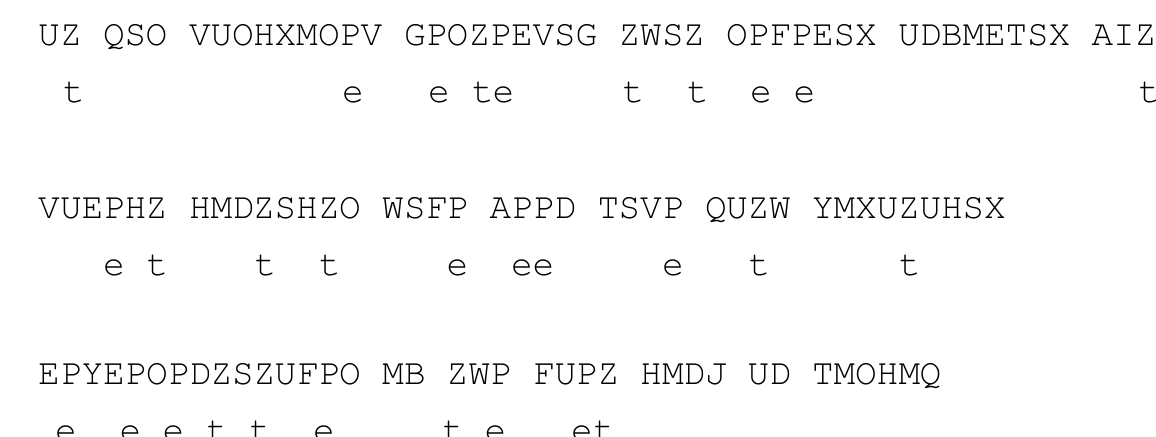
\includegraphics[width=126.42mm,height=119.99mm]{../../images/llm/page_016_img_01.png}%
\end{textblock*}

\end{document}
